\documentclass[11pt]{article}
\usepackage{newtxtext,newtxmath}
\usepackage{amsmath}%,amssymb}
\usepackage{geometry}
\usepackage{graphicx}
\usepackage{setspace}

% Packages for Polish language and character encoding
\usepackage[utf8]{inputenc} % For UTF-8 encoding
\usepackage[T1]{fontenc} % For proper hyphenation and accents in Polish

\thispagestyle{empty} 

\geometry{a4paper, left=15mm, right=15mm, top=20mm, bottom=10mm} % please to not change the margins

\usepackage[
   colorlinks,
   linkcolor=blue,
   urlcolor=blue,
   citecolor=blue,
   ]{hyperref}
   
\newcommand{\abstracttitle}[1]{
\setstretch{1.15}	%increase the space between the two lines of the title
 \begin{center}{\Large {\bf #1}}\end{center}
\setstretch{1.0}
}

\newcommand{\authors}[1]{
 \begin{center}{\bf #1} \end{center}
 \setstretch{1.0}
}

\newcommand{\addresses}[1]{
\setstretch{0.95}
 \begin{center}{\small #1} \end{center}
\setstretch{1}
}


\renewcommand{\thefootnote}{\fnsymbol{footnote}}
\newcommand{\writeto}[1]{
 \hspace*{-2.5mm} \footnote{\small E-mail: \href{mailto:#1}{#1}} %add \small= 10pt here
  \hspace*{-3.0mm} %decrease from -1.5 to -3.0mm
}


\renewcommand\refname{\normalsize References }

\begin{document}

\abstracttitle{The title of your contribution to OECS 19}
\authors{
B. Piętka $^{1,~}$\writeto{example@mail.com},
A. Opala $^{1}$,
P. Kapuściński$^{1}$,
M. Suster$^{2}$,
K. Tyszka$^{1}$,
P. Węgrzyn$^{2}$,
M. Matuszewski$^{3}$,
} 

\addresses{%Affiliation with laboratory and/or university name, city, zip code,  country
$^{1}$Faculty of Physics, University of Warsaw, ul.~Pasteura 5, 02-093 Warszawa, Poland \\
$^{2}$Candela Foundation, ul.~Grochowska 357/513, 03-822 Warszawa, Poland \\
$^{3}$Centre for Theoretical Physics, Polish Academy of Sciences,  al.~Lotników 32/46, 02-668 Warszawa, Poland
}


	Please follow these rules to ensure the happiness of the organizers and the beauty of the book of abstract: 
\begin{itemize}	
\item write your abstract in Times New Roman 11pt
\item indent the first line of each paragraph
\item do not exceed \textbf{\underline{1 page}}
\item include figures in the text with max. 2MB size
\item write the caption outside of the figure frame (see Figure~\ref{fig:Figure} as an example). 
\item insert your references using \textbackslash bibitem and cite as~\cite{AuthorsAB2024} and ~\cite{AuthorsCDE2023}
\item submit your abstract following procedure described at oecs19.pl
\end{itemize}

The nineteenth edition of the International Conference on Optics of Excitons in Confined Systems (OECS 19) is set to be held in Warsaw, Poland, from 14th to 18th July 2025. OECS, a conference convened every two years, serves as a platform for researchers engaged in the study of optical excitations in semiconductors, focusing particularly on excitons, polaritons, and collective excitations across various materials and photonic nanostructures. We extend our invitation for you to join us in Warsaw to explore the cutting-edge developments in this field of research.

    \begin{figure}[h]
    \begin{center}
        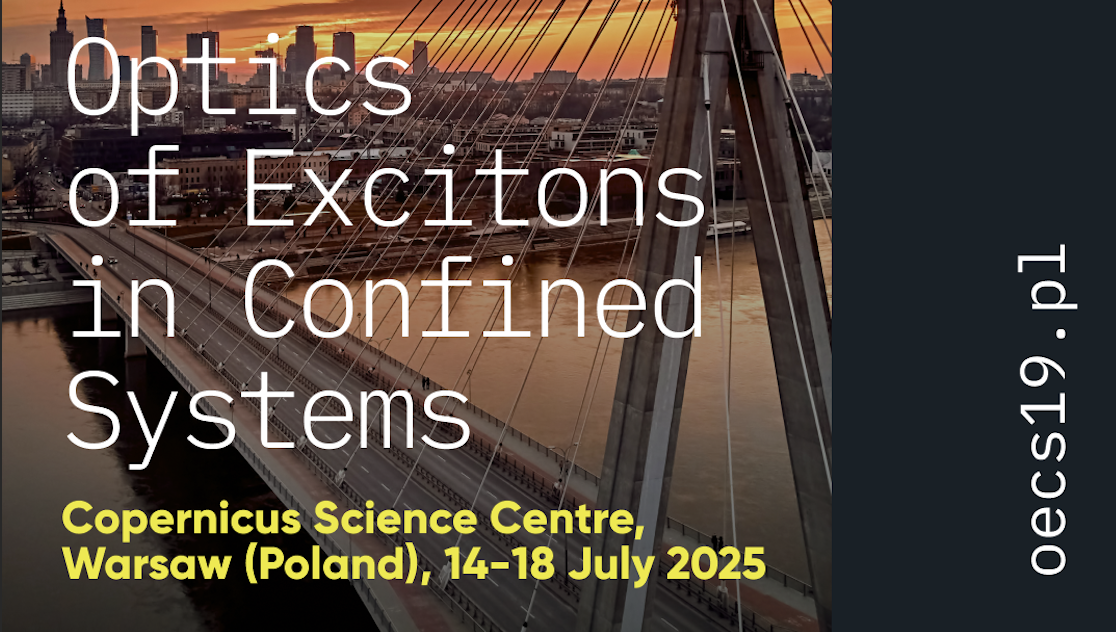
\includegraphics[width=0.4\textwidth]{images/Figure.png}
        \caption{\label{fig:Figure}
        Caption of your figure: Times New Roman, 11 points.}
    \end{center}    
    \end{figure}

\section*{\fontsize{11}{14}\selectfont Acknowledgments}
\vspace{-0.25cm}
\begin{flushleft}
\fontsize{11}{14}\selectfont % Adjust the line spacing if needed
Your acknowledgment text goes here.
\end{flushleft}


\begin{thebibliography}{1}
%insert your references here using \bibitem
\small
\vspace{-0.25cm}

\bibitem{AuthorsAB2024} N. White  and G. Black, {\em Nature Materials} {{\bf 6}, 9 (2024).} 
\vspace{-0.25cm} % Use this between every \bibitem to reduce the space between cited articles
\bibitem{AuthorsCDE2023} F. Bennett,  X.Y. Harrison, and  F. Foster, {\em Optica} {{\bf 15}, 11220 (2023).}

\end{thebibliography}
%\endgroup



\end{document}